\chapter{Inferring Unit Oracles from GUI Test Cases} \label{Chap:atrina}
%\javascript is extensively used in today's modern web applications. The close relation between the Document Object Model (DOM) and the underlying \javascript code creates an interactive web application. To check the application's behaviour from an end-user's perspective, testers often use popular frameworks such as Selenium. Using these frameworks to write DOM-based tests and assertions
%requires little knowledge about the internal operations performed at the client side code. Rather, the tester needs only basic knowledge of common event sequences to cover important DOM elements to assert. 
%This makes it easier for
%the tester to write DOM-based test suites. On the other hand,
%writing unit test assertions at code-level for web applications that have rich interaction with the DOM through their \javascript code is more tedious. 
%To write unit-level assertions, the tester needs to precisely understand the full range of interaction between the code level operations of a unit and the DOM level operations of a system, and thus may fail to assert the correctness of a particular behaviour when the unit is used as a part of a system. 
%
%Our previous findings \cite{mirshokraie:icst15} indicate that DOM-based assertions can potentially miss the related portion of
%code-level failure, while more fine grained unit-level assertions are capable of detecting such faults. Furthermore, finding the root cause of an error during DOM-based testing can be more expensive than during unit testing.
%The inherent characteristics of unit and DOM-based tests, indicate that they are complementary and that there is a trade-off in individually using each to detect faults. 
%
%Current test generation approaches either produce unit test oracles based on mutation testing techniques \cite{mirshokraie:icst15, fraser:tse12}, or they rely on soft oracles \cite{artzi:icse11}. Mutation-based approaches suffer from high computational cost and equivalent mutants which are syntactically different but semantically are the same as the original application.
%Soft oracles such as HTML validation and runtime exceptions are also limited in that they fail to capture logical and computational errors. 
%Recently, Milani Fard \etal \cite{milanifard:ase14} proposed using the DOM-based test suite of a web application to regenerate assertions for newly detected states through exploring alternative paths of the application. However, the new assertions generated by this technique remain at the DOM-level without considering the relation between the \javascript code and the DOM.
In response to our first research question (RQ 1.3.A), we propose to exploit an existing DOM-based test suite to generate unit-level assertions at the code-level for applications that highly interact with the DOM through the underlying \javascript code. We utilize
existing DOM-dependent assertions as well as useful execution information inferred from a DOM-based test suite to automatically generate assertions used for testing individual \javascript functions.

%To the best of our knowledge this work is the first to propose an approach for generating unit-level assertions by using the existing DOM-based test suite of the application. The main contributions of our work include:
%\begin{itemize}[noitemsep]
%\item A slicing-based technique to generate unit-level assertions capable of testing \javascript functions by utilizing existing DOM-based test assertions;
%\item A technique for selecting effective DOM elements in detecting code-level faults, which remain unchecked in the existing DOM-based test suite;
%\item An implementation of our approach in a tool, called \atrina; 
%\item An empirical evaluation to assess the efficacy of the approach on four open-source web applications;
Our approach is implemented in a tool, called \atrina.
The evaluation results show that the assertions generated by \atrina surpass the fault finding capability of (1) the human-written DOM-based assertions by 37\% on average, and (2) the state-of-the-art mutation-based assertion generation technique by 29\% on average.
%\end{itemize} 
\section{Challenges and Motivation} \label{Sec:motivation}
\figref{example} presents a snippet of a \javascript-based shopping cart application that we will use as a running example through out this paper. The application contains two main functions as follows:
\begin{enumerate}
\item \code{addToCart} is bound to the event handler of DOM elements with class \code{merchandise}. When the element is clicked, \code{addToCart} gets the information of the selected merchandise, and sets the quantity of the current available items by updating the \code{availItems} object. If a valid discount coupon exists, \code{addToCart} calculates the discount value, and disables the selected  coupon button with ID \code{couponButt} by removing the corresponding class. Finally, \code{addToCart} updates the payable amount by setting the \code{payable} property of the \code{customer} object.
\item \code{viewCart} is invoked by clicking on DOM element with ID \code{viewCart}. It shows a message containing the final payable amount of the customer. If the  coupon button with ID \code{couponButt} is not selected and the payable amount is equal to zero, then the empty cart message is shown.    
\end{enumerate}
%
%
%an expected value oracle for the given test input, confident
%that their effort is directed towards aspects of the system
%behavior that are relevant under that input
%
%easy to write DOM test and assert the final behaviour--difficult to write unit test and assert many intermediate behaviours that are also relevant to the final output. DOM-based tester may also miss some other important DOM-based behaviours to check.
%
%we can get more info from the sequence of events used in the dom-based test as the basis line of execution test + the dom-based assertion: from sequence we can infer missed dom checks. from dom-based assertion we can infer intermediate behaviours that are directly focused on the dom-based assertion + the rest of program points that are influenced by the assertion. this gives us an important set of oracles which falls in the neighbourhood area of the assertion, plus some important other oracles which are out of this neighbourhood zone but still important.  
\begin{figure}
%\medskip
\begin{lstlisting}
	var customer = {Id:"", couponStatus:"readyToUse", shopCart:"", ...};
	var coupon = {Id:"", ...}
	...
	$document.ready(function() {
		...
		$('#couponButt').click(selectCoupon);
	});
	
	function calculatePrice(customer, coupon) {
		coupElem = $('#couponButt');
		var price= $('#merchPrice').text();
		coupon.Id = couponFromServer(url + customer.Id);
		if(customer.couponStatus != 'used'){
			coupElem.removeClass(customer.couponStatus);
			customer.couponStatus = coupon.Id + '-' + 'used';
			discountVal = calcDiscount(coupElem.data('value'), customer.Id, coupon.Id);
			price -= discountVal;	
			coupElem.addClass(customer.couponStatus);
		} 	
		customer.shopCart = price;
		$('#calcPrice').text(price);  
	}
	
	function selectCoupon(){
		...
		customer.Id = customerFromServer($('#user').val());
		calculatePrice(customer, coupon);
	}

\end{lstlisting}
\vspace{-0.1in} 

\caption{\javascript code of the running example.}
\label{Fig:example}
\vspace{-0.2in} 

\end{figure} 


\section{Approach} \label{Sec:approach}
\begin{figure}[!t]
  \centering
  \includegraphics[width=1\hsize]{fig/approachDiagram}
  \vspace{-0.3in} 
  \mycaption{Overview of our assertion generation approach.}
  \label{Fig:approachDiagram}
  \vspace{-0.2in} 
\end{figure}
\IncMargin{0em}
\begin{algorithm}[t]
{\scriptsize
\SetKwInOut{Input}{input}\SetKwInOut{Output}{output}
\Input{Test suite $T$; The set of test cases $tc_i \in T$}
\Output{The ordered set of oracles $oracle$}
\BlankLine

\Begin {
\nl \For{$tc_i \in T$}{
\nl	 $trace\left textsc{Exec}(tc_i)$\\
\nl	 $domAccss\left \textsc{GetDomAcc}(trace)$   	


}

\caption{Oracle Generation} \label{Alg:algorithm}
}
\end{algorithm}
%\DecMargin{lem}
An overview of our unit-level assertion generation technique is depicted in \figref{approachDiagram}.
At a high level, our approach generates unit-level assertions by utilizing human written DOM-based tests and assertions. Our code level assertions fall in the following three categories: (1) explicit assertions, which are directly inferred from analyzing the manually written DOM-based assertions, (2) implicit assertions, which are indirectly affected by the human written DOM-based assertions, and (3) candidate assertions, which are not considered in the written DOM-based assertions, yet are potentially useful to be checked by the function level test suite. We describe our approach below. The numbers below in parentheses correspond to those in the boxes of \figref{approachDiagram}.

In the first part of our approach we (1) execute the instrumented application by running the existing DOM-based test suite. In this step we gather a detailed execution trace of the application. We then extract (2) DOM-based assertions, and (3) candidate DOM element properties, which are useful DOM properties that can potentially be utilized for the purpose of assertion generation. We (4) identify the initial point of connection between the application's source code and checked DOM element. 
%We collect lines of code responsible for updating the corresponding DOM element. 
%We determine DOM mutating statements, 
We (5) calculate the backward slice of the DOM mutating statements to find the entire code blocks that update the checked DOM element. We then (6) extract accessible entities from the obtained statements. Accessible entities form our explicit assertions (7). We further (8) perform a forward slice on the extracted entities to identify statements, that are implicitly affected by such entities. The accessible entities associated with the collected statements form our implicit assertions (9). In addition to explicit and implicit assertions, we also generate candidate assertions (10). Candidate assertions are involved with updating potentially useful DOM element properties, which are not checked in the existing DOM-based assertions. To obtain candidate assertions, we perform step (4), (5), and (6) on the inferred candidate DOM element properties (3).

Our overall unit-level assertion generation is presented in \algref{algorithm}. In the following sections we describe our technique for extracting DOM related information from the execution (\secref{extractDomRelatedInfo}), relating
DOM mutations to the \javascript code (\secref{domToCode}), and generating unit test assertions (\secref{unitLevelAssertion}).   
\subsection{Extracting DOM-Related Characteristics} \label{Sec:extractDomRelatedInfo}
The DOM connects a test case to the web application's code. Therefore, we first need to analyze the DOM-based test suite and extract the following pieces of information: (1) DOM-related operations of the existing test suite that may have tight connection with the \javascript code, and (2) frequently accessed DOM properties, which are potentially influential in improving the fault finding capability of the test suite, but left unchecked in the manually-written test suite.
\headbf{DOM-Related Operations}
Any written test case needs to check the correctness of the application's behaviour. In a DOM-based test case the expected behaviour is checked through DOM-based assertions.
DOM-based assertion is defined as $<domProps,expVal>$, where $domProps$ consists of one or more DOM element features (e.g. attribute, and/or textual value), and $expVal$ is the correct value expected by the assertion. Through the rest of the paper, we call DOM element feature as DOM property. 
DOM-based assertions play a significant role in our approach as they can guide us towards important portions of the underlying \javascript code that need to be checked in unit-level assertions.
\begin{figure}[!t]
  \centering
  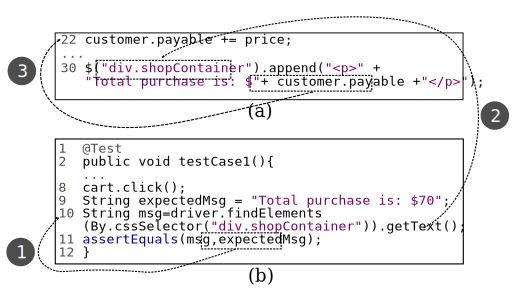
\includegraphics[width=1\hsize]{fig/intraDOMDep}
   \vspace{-0.2in} 
  \mycaption{Finding (1) intra DOM assertion dependency within the test case (b), (2) inter DOM assertion dependency between (b) DOM-based assertion and (a) the \javascript code, and (3) the initial point of contact between (b) DOM-based assertion and (a) the \javascript code.}
  \label{Fig:assertionToCode}
%  \vspace{-0.1in} 
\end{figure}
For each DOM-based assertion we find \emph{intra DOM assertion dependency} within the test case.
\begin{mydef}[Intra DOM Assertion Dependency]
An intra DOM assertion dependency is defined as $<assert, domElems, domProps>$, where $assert$ is the intended DOM-based assertion, $domElems$ is the accessed DOM elements in the test case pertaining to the assertion, and $domProps$ is the accessed DOM properties within the assertion.
\end{mydef}
\textsc{GetDomAcc} in line 10 of \algref{algorithm} retrieves DOM dependencies of the assertion in the test case.
%, we instrument the test case by wrapping around method calls that accesses DOM elements.
Going back to our example in \figref{assertionToCode}(b), tracking the assertion in line 11 shows that it has a DOM dependency to a \code{div} element with class \code{shopContainer}, which is accessed in line 10. The intra DOM assertion dependency of the example further shows that the \code{text} value of the DOM element is compared with the \code{expectedMsg} in line 11.    

We further need to correlate the inferred intra DOM assertion dependency with the application's code.
We call the correlation between the DOM-based assertion and the application's code as \emph{inter DOM assertion dependency}.
\begin{mydef}[Inter DOM Assertion Dependency]
An inter DOM assertion dependency is defined as\\
$<assert, initPoint>$, where $assert$ is the intended DOM-based assertion, and $initPoint$ is the initial line of code in the application that is responsible for mutating the property of a DOM element extracted from the intra DOM assertion dependency.
\end{mydef}
In order to find the initial point of contact between the application's code and a mutated DOM property in the DOM-based test case, we track evolution of the accessed DOM elements (\textsc{GetDomMuts} in line 13 of the algorithm) as well as invoked event handlers as the test case runs. 
We consider additions and removals of child nodes, changes to attributes, and updates to child text nodes as DOM mutations. For instance, running the sample test case in \figref{example}(b) results in mutating (1) the textual value of \code{div} element with class \code{shopContainer}, and (2) the \code{class} attribute of DOM element with ID \code{couponButt}.

In \secref{domToCode}, we explain inferring the initial point of contact between the source code and a mutated DOM element in a DOM-based test suite in details.  
%We call the correlation between the DOM-based assertion and the \javascript code of the application as \emph{inter DOM assertion correlation}. This correlation is defined as $<AccDOMDep, InitCode>$, where $InitCode$ is the initial point of contact in the application's code segment, that is responsible for mutating the previously extracted DOM elements from the test suite ($AccDOMDep$).  
%We make use of \code{document.onload} event to log the initial DOM state. 
%An observer module is then used to monitor mutations on the DOM during the test case execution. 
%In addition to DOM changes, we also keep track of \javascript events as well as invoked event handlers. This information is later used to find the initial point of contact between a DOM mutation and the executed code segments.
%For instance, running the sample test case in \figref{example}(b) results in mutating (1) the textual value of \code{div} element with class \code{shopContainer}, and (2) the \code{class} attribute of DOM element with ID \code{couponButt}.
\headbf{Frequently Accessed DOM Properties}
In addition to DOM-based assertions, we further consider DOM element properties, that are frequently accessed within the application as the test case runs (lines 1 to 7 of \algref{algorithm}). 
\textsc{Acc} in line 6 of the algorithm computes the access frequency of a DOM property, $freqAccdDOM$ in line 7 contains the inferred candidate DOM properties, and \textsc{GetDomMuts} in line 19 records DOM mutations occur
on candidate DOM properties.
The intuition is that frequent use of a given DOM property can point to the extent of application's behaviour dependency on the DOM property. Thus, if changes happen to that property through the \javascript code, it is important to assert the correctness of such mutations. We define the access frequency of a DOM element property as the number of times that the element's property has been read during the execution of a test case. DOM properties include attributes as well as textual value of the elements.
In order to record DOM property accesses within the application, we rewrite native function calls used by programmers to access DOM element such as \code{getElementById}, \code{getElementsByClassName}, and/or \code{getElementsByTagName}. The returned object from these functions is later used to access attributes or textual values of the element. Thus, we apply a forward slice on the returned object to find instances of element's property access in the code.
For example in function \code{addToCart} of \figref{example}(a), DOM element with ID \code{couponButt} is assigned to \code{coupElem} variable. The assigned variable is later used to access the \code{class} attribute as well as the \code{value}
of the DOM element in lines 23, 25, and 26.

Let $Acc(prop_{el})$ be the access frequency computed for property $prop$ of DOM element $el$, then:
 
$Acc(prop_{el})=\frac{Read(prop_{el})}{\sum _{e=1}^{n} Read(domElem_e)}$, where $Read(domElem_{e})$ is the number of times that DOM element $domElem$ is read, given that the total number of DOM elements during the execution of a test case is $n$.
Note that reading a DOM element refers to accessing the element to read the corresponding property. In \figref{example}(a), the \code{class} attribute of DOM element \code{couponButt} is read in lines 23 and 34, and thus the access frequency
computed for the \code{class} attribute of the element is equal to $\frac{2}{3}$.

We choose element's property with access frequencies above a threshold $\alpha$ as potential candidates, which are later used for the purpose of unit-level assertion generation. We automatically compute this threshold for each test case as: 

$\alpha=\frac{1}{ReadProperties(T)}$, where $ReadProperties(T)$ is the total number of properties which have been read during the execution of test suite $T$.

Going back to our running example and the sample DOM-based test case in \figref{example}, \code{class} attribute of the \code{couponButt} is selected as a potential candidate since its access frequency ($\frac{2}{3}$) is greater than the computed threshold, which is equal to $\frac{1}{2}$ in this example.        
%application instrumentaion native event wrapping    

\subsection{Relating DOM changes to the \javascript Code} \label{Sec:domToCode}
To determine the initial point of contact between DOM and the underlying \javascript code, we first cross reference the relevant DOM element with a set of DOM mutations obtained from the execution trace. Our execution trace contains information about the invoked functions, triggered events, as well as DOM mutations caused by the events as the test case runs. This way we can identify relevant events and functions corresponding to a DOM mutation. To figure out where the mutation originated in our execution trace we keep record of DOM accesses within the application. For each DOM access we track \javascript lines of code, that are responsible for updating the corresponding DOM element. After inferring DOM mutant statements within the code, we perform backward slice on the retrieved statements to gather the entire set of \javascript statements responsible for mutating a given DOM element. 
In order to capture dependencies exercised at run-time we use dynamic slicing. We first intercept and statically instrument those statements that may affect a given DOM element. The instrumented code keeps track of all updates and accesses to all relevant data and control dependencies. This trace is later used to extract a dynamic backwards slice.    
Once the test case runs, we collect traces from the instrumented code. This trace is used for extracting dynamically backward sliced statements.

The slicing technique starts by extracting instances of the initial slicing criteria from the trace. For each \textit{read} operations, the trace is traversed backwards to find the nearest related \textit{write} operation. Once found, the \textit{write} operation is added to the slice under construction. This process is repeated for all the data dependencies related to that write operation. A similar approach is taken for including control dependencies in the slice.
To address aliasing when computing the slice of a variable that has been set by a non-primitive value, we need to consider possible aliases that may refer to the same object. Specifically in \javascript \textit{dot notation} and \textit{bracket notation} is frequently used to modify objects at run time. While static analysis techniques often ignore addressing this issue \cite{Feldthaus:icse13}, we incorporate dynamic analysis in our slicing method. If a reference to an object of interest is saved to a second object's property, e.g. through the use of the \textit{dot notation}, the object of interest may also be altered via aliases of the second object. For example, after executing statement \code{a.b.c = objOfInterest;}, updates to \code{objOfInterest} may be possible through \code{a}, \code{a.b}, or \code{a.b.c}. To deal with such scenarios, our slicing technique searches through the collected trace and adds the forward slice for each detected alias to the current slice for our variable of interest (e.g. \code{objOfInterest}). 

By the end of backward slicing step we collect all the relevant statements to a given DOM element, which re later used to derive test assertions.    
\subsection{Generating Unit-Level Assertions} \label{Sec:unitLevelAssertion}
Through analyzing a given DOM-based test case, we generate unit-level assertions in the following three categories: (1) assertions, which are directly related to a given DOM-based assertion, (2) assertions, which are indirectly affected by a given DOM-based assertion, and (3) assertions that have direct impact on important DOM elements which are not checked by the existing DOM-based assertions. In the following we explain each category in details.
\subsubsection{Explicit Assertions} \label{Sec:explicitAssertions}
After collecting all the statements, that are relevant to a given DOM-based assertion, we extract accessible entities from these statements.
Accessible entities include (1) the function's returned value, (2) the used global variables in that function, (3) the object's property where the object is accessible in the outer scope of the function, and/or (4) the accessed DOM element in that function. Dynamic backward slice of a DOM-based assertion helps to (1) track all statements that contribute to the checked result and as such identify those entities that might have influenced the checked property value of the DOM element, and (2) eliminate unrelated entities which are not involved in the computation that leads to the update performed on the checked DOM element.

Since our dynamic slice is extracted from the program run, we can track all concrete values associated with accessible entities.
During the run of a test case, there might be different instances where a given statement is executed. Different execution instances can lead to different behaviour. Since we are employing dynamic slicing, an instance that leads to the required behaviour, which is verified through the DOM-based assertion, is on the backward slice. Given that the manually-written expected value, that is checked against the DOM's property is valid, the concrete values of related entities in the backward slice are potentially correct unless there exists a masked fault which is concealed in the chain of computations and thus does not propagate to the checked state of the DOM element. We conjecture that fault masking rarely happens in \javascript web applications as it is more prevalent in programs with many small expressions whose results are stored in several intermediate values (we further discuss this in the evaluation section). Therefore, concrete value of an entity in the backward slice can potentially be used as the expected value of the entity in unit-level assertions to test the current version of the application.
%We compare the value of the entity immediately after the relevant statement is executed in the backward slice with the entity's value before the function exits. If value of the entity remains the same, we use it towards the expected value in the unit-level assertion.  
%However, if the entity pertaining to a DOM change is reassigned in the code after the DOM gets updated and before the function exits, then the concrete value of the entity can be used for the purpose of regression testing unless the tester provides the proper expected value.
\subsubsection{Implicit Assertions} \label{Sec:implicitAssertions}
We gather all the statements that explicitly affect the computations relevant to a given DOM-based assertion. While assertions inferred from such statements are inherently important, we further need to consider entities that are implicitly influenced by the checked DOM element in the manually-written test suite. For this purpose we apply a dynamic forward slice on the statements collected from a backward slice of a DOM-based assertion.
%\begin{mydef}[Forward Slicing]
%\label{def:forwardSlicing} 
%A forward slice of a program with respect to a statement $st$ at program point $p$ and set of program variables $V$ consists of all statements and predicates in the program that are affected by the value of variables in $V$ at $p$.
%\end{mydef}
A forward slice with respect to a statement $st$,
indicates how subsequently an operand at $st$ is being used. This can help the tester to ensure that $st$ establishes the expected outcome of the computations assumed by later statements. 
%Given the importance of statements involved in code-level computations of a DOM-based assertion, using forward slice is useful to check that there are no unforeseen effects on the application's behavior by a modification to such statements. 

\begin{figure}[!t]
  \centering
  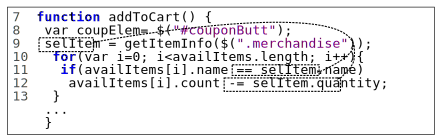
\includegraphics[width=1\hsize]{fig/forwardSlicingExample}
   \vspace{-0.2in} 
  \mycaption{Forward Slicing to obtain implicit assertions.}
  \label{Fig:forwardSlicingExample}
 % \vspace{-0.1in} 
\end{figure}

Dynamic forward slice is performed on the subset of code statements which is previously instrumented as explained in \secref{domToCode}. 
\textsc{GetFWSlice} in line 17 of the algorithm computes forward slice on the variable operands of a statement in the backward slice.
The process of forward slicing is similar to the backward slicing technique discussed earlier (\secref{domToCode}). The slicing criterion of the forward slice module is either a variable, object's property, or an accessed DOM property extracted from the statements in a backward slice segments of the code. The accessible entities (\textsc{Accessibles} in line 24), which have been set within the collected forward slice statements establish the implicit assertions.
$implicitAsstn$ in line 24 of \algref{algorithm} contains the inferred implicit assertions.
\figref{forwardSlicingExample} shows the relevant parts of the code obtained by performing forward slicing on the running example. 
As shown in the figure, the properties of object \code{selItem} are set in line 16, that is recorded during the backward slice process. Given line 16 as the forward slice criteria, we mark \code{availItems.count} (line 19) as an implicit assertion.        
\input{potentialAssertions}
          
%mutation of customer.couponStatus = coupon.Id + '-' + 'used' to customer.couponStatus = coupon.Id + 'used';'
\subsection{Tool Implementation} \label{Sec:tool}
We have implemented our \javascript test and oracle generation approach in an automated tool called \tool. The tool is written in Java and is publicly available for download \cite{jseft-dl}. Our implementation requires no browser modifications, and is hence portable. For \javascript code interception, we use a web proxy, which enables us to automatically instrument \javascript code before it reaches the browser. 
The crawler for \tool extends and builds on top of the  event-based crawler, \crawljax \cite{mesbah:tweb11}, with random input generation enabled for  form inputs.
%
As mentioned before, to mutate \javascript code, we use our recently developed mutation testing tool, \mutandis \cite{mirshokraie:icst13}. The upper-bound for the number of mutations can be specified by the 
user. However, the default is 50 for code-level and 20 for DOM-level mutations. We observed that these default numbers  provide a balanced trade-off between oracle generation time, and the fault finding capability of the tool. %In the current implementation of \tool, we ignore semantic equivalence in the DOM, meaning that we assume that any modification to the DOM is potentially an undesirable behaviour from the tester's perspective.
 % 
 %To instrument the intercepted code, Mozilla Rhino \cite{rhino} is used to parse \javascript code to an AST, and back to the source code after the instrumentation is performed. %We use Rhino's APIs to search for program points where instrumentation code needs to be added. 
%To generate DOM-level event-based tests, %we extend our previously developed test generation plugin\curl{https://github.com/crawljax/testcasegenerator-plugin/} \cite{mesbah:tse12} in 
%
DOM-level test cases are generated in a \junit format that uses \selenium (WebDriver) APIs to fire events on the application's DOM inside the browser. \javascript function-level tests are generated in the \qunit unit testing framework \cite{quint}, capable of testing any generic \javascript code. 


\section{Empirical Evaluation} \label{Sec:evaluation}

To quantitatively assess the efficacy of our mutation testing approach, we have conducted a case study in which we address the following research questions:

\begin{description}
\item [RQ1] How efficient is \mutandis in generating non-equivalent mutants?
%\item [RQ2] How effective is \codename in injecting critical behaviour-affecting faults?
\item [RQ2] How effective are $FunctionRank$ and selective variable mutation in (i) generating non-equivalent mutants, and (ii) injecting non-trivial behaviour-affecting faults?
\item [RQ3] How useful is \mutandis in assessing the existing test cases of a given application?

\end{description} 

The experimental data produced by \mutandis is available for download.\footnoterecall{mutandisDownload}

\begin{table*}
\centering
%\vspace{5pt}
        \caption{Characteristics of the experimental objects.}
{\scriptsize
    \begin{center}
       
      %  \subtable[Experimental subjects and the corresponding exploration data]
            {
           \begin{tabular}{c|l|c|c|c|l} \hline
\theadturn{App ID} &\theadturn{Name} &\theadturn{JS LOC} & \theadturn{\# Functions} &\theadturn{CC} &\thead{Resource}  \\  \hline \hline

1  & SameGame & 206 & 9 & 37 & \url{http://crawljax.com/same-game}   \\ \hline
           
2 & Tunnel & 334 & 32  & 39 & \url{http://arcade.christianmontoya.com/tunnel} \\ \hline

3 & GhostBusters & 277 & 27 & 52 & \url{http://10k.aneventapart.com/2/Uploads/657}  \\ \hline

4 & Symbol & 204 &  20 & 32  & \url{http://10k.aneventapart.com/2/Uploads/652}\\ \hline

5 & TuduList & 2767 &  229 & 28  & \url{http://tudu.ess.ch/tudu}\\ \hline

6 & SimpleCart (library) & 1702 & 23  &  168 & \url{http://simplecartjs.org}\\ \hline

7 & \jquery (library)& 8371  &  45 & 37  & \url{https://github.com/jquery/jquery}\\ \hline

8 & WymEditor & 3035  &  188 & 50  & \url{https://github.com/wymeditor}\\ \hline

\hline\end{tabular}\centering
            }
\label{Table:objectsChar-table}
\end{center}
}  
\vspace{-0.1in} 
\end{table*}


\subsection{Experimental Objects}
Our study includes eight \javascript-based objects in total. Four
are game applications, namely, SameGame, Tunnel, GhostBusters, and Symbol. One is  a web-based task management application called TuduList. Two, namely SimpleCart and \jquery, are \javascript libraries. The last application, WymEditor, is a web-based HTML editor. All the experimental objects are open-source applications.
One of our main inclusion criteria was for the applications to extensively use \javascript on the client-side.
Although the game applications used in our study are small size web applications, they all extensively and in many different ways use \javascript.

%
\tabref{objectsChar-table} presents each application's ID, name, and resource, as well as the static  characteristics of the \javascript code, such as \javascript lines of code (LOC) excluding libraries, number of functions, and the cyclomatic complexity (CC) across all \javascript functions in each application.

\begin{table}
%\vspace{5pt}
        \caption{Bug severity description.}
{\scriptsize
    \begin{center}
       
      %  \subtable[Experimental subjects and the corresponding exploration data]
            {
           \begin{tabular}{l|l|l} \hline
\thead{Bug Severity} &\thead{Description} &\thead{Rank}  \\  \hline \hline

Critical  & Crashes, data loss & 5   \\ \hline
Major  & Major loss of functionality & 4   \\ \hline
Normal  & Some loss of functionality, regular issues & 3   \\ \hline
Minor  & Minor loss of functionality & 2   \\ \hline
Trivial  & Cosmetic issue & 1   \\ \hline

\hline\end{tabular}\centering
            }
\label{Table:bugSeverity-table}
\end{center}
}  
\vspace{-0.1in} 
\end{table} 


\subsection{Experimental Setup}
To run the analysis, we provide the URL of each experimental object to \mutandis. 
Note that because SimpleCart and \jquery are both \javascript libraries, they cannot be executed independently. However, since they come with test cases, we use them to answer RQ3.
%we are not able to use them in response to RQ1 and RQ2, as they are not independently executable. 
%As a result, we use them to answer RQ4. %The first five applications are used for answering RQ1--RQ3.

We evaluate the efficiency of \mutandis in generating non-equivalent mutants (\textbf{RQ1}) for the first five applications in \tabref{objectsChar-table}. 
We collect execution traces by instrumenting the custom \javascript code of each application and executing the instrumented code through automated dynamic crawling. 
We navigate each application several times with different crawling settings. Crawling settings differ in the number of visited states, depth of crawling, and clickable element types.
We inject a single fault at a time in each of these five applications using \mutandis. The number of injected faults for each application is 40; in total, we inject 200 faults for the five objects. We automatically generate these mutants from the following mutation categories: (1) variables, (2) branch statements, and (3) \javascript-specific operators. We then examine each application's behaviour to determine whether the generated mutants are equivalent.  

The determination of whether the mutant is equivalent is semi-automated for observable changes.
An observable change is a change in the behaviour of the application which can be observed as the application is automatically executed in the browser.
Note that in web applications DOM is an observable unit of the application, which is shown in the browser. We execute the same sequence of events in the mutated version as it is used in the original version of the application. The resulting observable DOM of the mutated version in the browser is visually compared against the original version. 
%as we automatically execute the mutated version of the application in the browser. 
If we notice any observable change during the execution, the mutant is marked as non-equivalent. 
This way we can eliminate the burden of manual analysis of the applications' source code for every mutants.  
For non-observable changes, we manually inspect the application's source code to determine whether the mutant is equivalent.
%\karthik{How is executing the application in the browser enough to detect observable changes ? Do we not need someone to observe the difference ?}

To make sure that changes in the applications' behaviour, from which the non-equivalency is determined, are not cosmetic changes we use the bug severity ranks used by Bugzilla, a popular bug
tracking system. %which have also been used by other researchers \cite{bhattacharya:icse12}. 
The description and the rank associated with each type of bug severity is shown in \tabref{bugSeverity-table}. We choose non-equivalent mutants from our previously generated mutants (for RQ1). We then analyze the output of the mutated version of the application and assign a bug score according to the ranks in \tabref{bugSeverity-table}.

To address \textbf{RQ2}, we measure the effectiveness of \mutandis in comparison with random-based mutation generation. Moreover, to understand the impact of applying $FunctionRank$ and rank-based variable mutation in generating non-equivalent mutants as well as injecting behaviour-affecting faults we compare:
\begin{enumerate} [noitemsep, nolistsep]
\item The proposed $FunctionRank$ metric with $PageRank$;
\item Our selective variable mutation with random variable mutation;
\end{enumerate}
Similar to RQ1, we use the ranks provided by Bugzilla to measure the criticality of the injected faults on the non-equivalent mutants.  

Unfortunately, no test suites are available for the first five applications.  Thus, to address \textbf{RQ3}, we run our tool on the SimpleCart, \jquery, and WymEditor that come with Qunit\curl{http://docs.jquery.com/QUnit} test cases. We gather the required execution traces of the SimpleCart library by running its test cases, as this library has not been deployed
on a publicly available application. However, to collect dynamic traces of the \jquery library, we use one of our experimental objects (SameGame), which uses \jquery as one of its \javascript libraries. Unlike the earlier case, we include the \jquery library in the instrumentation step. We then analyze how the application uses different functionalities of the \jquery library using our approach. The execution traces of the WymEditor are collected by crawling the application. We generate 120 mutants for each of the three experimental objects. Mutated statements, which are not executed by the test suite are excluded. After injecting a fault using \mutandis, we run the test cases on the mutated version of each application. 
We determine the usefulness of our approach based on (1) the number of non-equivalent generated mutants, and (2) the number of non-equivalent \emph{surviving} mutants.  A non-equivalent surviving mutant  is one that is neither killed nor equivalent, and is an indication of the incompleteness of the test
cases. The presence of such mutants can help testers to improve the quality of their test suite. 
For mature test suites, we expect the number of non-equivalent surviving mutants to be low \cite{raise:jalbert12}. We further compare \mutandis against random mutation testing to evaluate the effect of our approach on the stubbornness of the generated mutants. Stubborn mutants are non-equivalent mutants that remain undetected by a high quality test suite \cite{yao:icse14}.

\begin{table*}
%\vspace{5pt}
        \caption{Mutants generated by \mutandis.}
{\scriptsize
   
       \begin{center}
      %  \subtable[Experimental subjects and the corresponding exploration data]
            {
          \begin{tabular}{l|l|l|l|l|l|l} \hline
\thead{Name} & \thead{\# Mutants} & \thead{\# Equiv Mutants} & \thead{\# Non-Equiv Mutants} & \thead{Equiv Mutants (\%)} & \thead{Bug Severity Rank (avg)} & \thead{Bug Severity (\%)} \\  \hline \hline

  SameGame & 40 & 2 & 38 & 5.0 & 3.9 & 78\\ \hline
  Tunnel & 40 & 4 & 36 & 10.0 & 3.8 & 76\\ \hline
  GhostBusters & 40 & 3 & 37 & 7.5 & 3.2 & 64\\ \hline
  Symbol & 40 & 3 & 37 & 7.5 & 3.9 & 78 \\ \hline
  TuduList & 40 & 2 & 38 & 5.0 & 3.8 & 76\\ \hline 
 Avg. & 40 & 2.8  & 37.2  & 7.0 & 3.7  & 74.4 \\ \hline
  

\hline \end{tabular}\centering
            }

\label{Table:bugSeverity-equiv-table}
\end{center}
}  
\vspace{-0.1in} 
\end{table*}

\subsection{Results}
%In this section, we discuss the results of the case study with regard to our three research questions.
\head{Generated Non-Equivalent Mutants (RQ1)} \tabref{bugSeverity-equiv-table} presents our results for the number of non-equivalent mutants and the severity of the injected faults using \mutandis.
For each web application, the table shows the number of mutants, number of equivalent mutants, the number of non-equivalent mutants, 
the percentage of equivalent mutants, and the average bug severity as well as the percentage of the severity in terms of the maximum severity level. 
%$\left(\frac{\#Non-EquivMutants}{\#TotalMutants}\right)\times 100$

As shown in the table, the number of equivalent mutants varies between 2--4, which corresponds to less than 10\% of the total number of mutants.%, which compares favourably to other techniques that have observed the number of equivalent mutants to be between 10 to 40\%.

\answer{On average, the percentage of equivalent mutants generated by \mutandis is  7\%, which points to its efficiency in generating non-equivalent mutants.} 

We observe that more than 70\% of these equivalent mutants generated by \mutandis originate from the branch mutation category. The reason is that in our current approach, branch expressions are essentially ranked according to the variables used in their expressions without considering whether mutating the expression changes the actual boolean outcome of the whole expression (e.g.; \code{if(trueVar || var)\{...\}} where the value of \code{trueVar} is always \code{true}, and thus mutating \code{var} to \code{!var} does not affect the boolean outcome of the expression). We further notice cases in our experimental objects where the programmer writes essentially unused hard-coded branch expressions.
%This can result in mutating a branch that does not affect the application's behaviour. 
For instance, in Tunnel, we observed a couple of \code{return true/false} statements at exit point of the functions that have high $FunctionRank$ and cyclomatic complexity value. However, the returned value is never used by the caller function and hence, mutating the return boolean value as part of branch mutation generates an equivalent mutant. This is the main reason that we observe 10\% of equivalent mutants (the highest in \tabref{bugSeverity-equiv-table}) for the Tunnel application. Moreover, we notice that certain types of mutation operators affect the number of equivalent mutants. For example for a number of mutations we observe that replacing $>=$ ($<=$) sign with $>$ ($<$) keeps the program's behaviour unchanged since either the lower/upper bound is never reached or the programmer specify extra bounds checking before returning the final value.
  
%As far as RQ1 is concerned
%our tool is capable of automatically generating mutants, which are not equivalent with high probability.
\headbf{Fault Severity of the Generated Mutants} The fault severity of the injected faults
is also presented in \tabref{bugSeverity-equiv-table}. We computed the percentage of the bug severity as the ratio of the average severity rank to the maximum severity rank (which is 5). As shown in the table, the average bug severity rank across all applications is 3.72 (bug severity percentage is 74.4\% on average).
%This indicates that the injected faults cause normal to major loss of functionality.
%Based on \tabref{bugSeverity-table}, we see that: 
%
%\answer{Based on an average severity rank of 3.72, the injected faults cause normal to major loss of functionality.}
%
We observed only a few faults with trivial severity (e.g; cosmetic changes).
We also noticed a few critical faults (3.8\% on average), which caused the web application to terminate prematurely or unexpectedly.
It is worth noting that full crashes are not that common for web applications, since web browsers typically do not stop executing the entire web application when an error occurs. The other executable parts of the application continue to run in the browser in response to user events \cite{Ocariza-2011}. 
Therefore, it is very rare for web applications to have type 5 errors, and hence the maximum severity rank is often 4.
%Further, we made the following important observation for all the applications:

\answer{More than 70\% of the injected faults causing normal to major loss of functionality are in the top 20\% ranked functions, showing the importance of $FunctionRank$ in the fault seeding process.}

Moreover, we noticed that the careful choice of a variable for mutation is also as important as the function selection. For example, in the SameGame
application, the \code{updateBoard} function is responsible for redrawing the game board each time a cell is clicked. Although \code{updateBoard}
is ranked as an important function according to its $FunctionRank$, there are two variables within this function that have
high usage frequency compared to other variables. While mutating either of these variables causes major loss of functionality, 
selecting the remaining ones for mutation either has no effect or only marginal effect on the application's behaviour.
Furthermore, we observed that the impact of mutating variables that are part of the invariants as well as the variables 
with high usage frequency can severely affect the application's behaviour. This indicates that both invariants and usage
frequency play a prominent role in generating faults that cause major loss of functionality, thereby justifying our choice
of these two metrics for variable selection (Section~\ref{variable-ranking}).   
%
%As far as RQ2 is concerned, our results indicate that \mutandis is effective in generating mutants that cause non-trivial errors in \javascript applications.


\begin{figure}[!t]
  \centering
  \includegraphics[width=0.7\hsize]{r-scripts/equivMuts-barPlot}
  \vspace{0.09in} 
  \mycaption{Equivalent Mutants (\%) generated by \mutandis, random, PageRank, and random variable selection.}
  \label{Fig:equivMuts-barPlot}
\end{figure}

\begin{figure}[!t]
  \centering
  \includegraphics[width=0.7\hsize]{r-scripts/bugSeverity-barPlot}
  \vspace{0.09in} 
  \mycaption{Bug Severity Rankd (Avg) achieved by \mutandis, random, PageRank, and random variable selection.}
  \label{Fig:bugSeverity-barPlot}
\end{figure}

\head{Effectiveness of $FunctionRank$ and selective variable mutation (RQ2)} \label{Sec:eval-comparison}

The results obtained from \mutandis, random mutation, $PageRank$, and random variable mutation %(1) \mutandis with random mutation, (2) $FunctionRank$ with $PageRank$, and (3) selective variable mutation with random  variable mutation, 
 in terms of the percentage of equivalent mutants and bug severity rank are shown in \figref{equivMuts-barPlot} and \figref{bugSeverity-barPlot}, respectively.



As shown in \figref{equivMuts-barPlot}, the percentage of equivalent mutants generated by \mutandis is always less than or equal to the ones generated by the other three approaches. 
Not surprisingly, random mutation obtains the largest percentage of equivalent mutants (ranges from 7.5--15\%). 
This indicates that our selective variable mutation plays a more prominent role in reducing the percentage of equivalent mutants generated by \mutandis.


\answer{On average, \mutandis reduces the number of equivalent mutants by 39\% in comparison with random mutation generation.}

\answer{On average, $FunctionRank$ and selective variable mutation reduce the number of equivalent mutants by 12\% and 26\%, respectively when compared with $PageRank$ and random variable mutation.}

We observed that for three applications (ID=1, 2, 4) the main reason behind the reduction in the number of equivalent mutants is the use of selective variable mutation, 
as by replacing selective variable mutation with random mutation,
the percentage of equivalent mutants significantly increases (ranges from 33--50\% increment)
For these applications, we observed that although high rank functions are selected for mutation, modifying a non-behavioural affecting part of the selected function's code (\ie a useless branch or variable) results in generating an equivalent mutant. Therefore, the choice of the variable or branch to mutate is very important.

However, for application with ID 3 (GhostBusters), $FunctionRank$ plays a prominent role in reducing the number of equivalent mutants.
\figref{equivMuts-barPlot} shows that for this application the percentage of equivalent mutants becomes the same as \mutandis, when we use random variable mutation coupled with $FunctionRank$. 
We observed that in the aforementioned application,
major variables in the program have high usage frequency. Moreover, these variables are shared among detected invariants, thus making the selection of a specific variable for mutation less
effective compared to other applications. For the last application (ID 5), we observed that $FunctionRank$ and selective variable mutation are both effective in terms of generating
non-equivalent mutants.

\figref{bugSeverity-barPlot} compares the severity of the injected faults according to the ranks provided in \tabref{bugSeverity-table}. The results show that \mutandis achieves the highest rank among the other approaches. Our mutation generation technique increases the criticality of the injected faults by 20\% in comparison with random mutation approach. 
%
%\answer{Our approach increases the criticality of the injected faults by 20\% in comparison with random mutation approach.}

We observed that by replacing $FunctionRank$ with $PageRank$, the severity of the behaviour-affecting faults drops by 13\%, which indicates that $FunctionRank$ outperforms $PageRank$ in terms of its impact on the behaviour of the application towards more critical failures.
%
%\answer{$FunctionRank$ outperforms $PageRank$ in terms of its impact on the behaviour of the application towards more critical failures.} 

We further noticed that using the proposed selective variable mutation increases the bug severity by 9\% on average. While this indicates the importance of
using the proposed variable mutation technique, it reveals that our rank-based function selection technique plays a more prominent role in increasing the severity degree of the injected faults compared to our variable selection strategy.
For example, in application with ID 2 (Tunnel), function \code{updateTunnel} contains the main logic of the application, and it is among the top-ranked functions.
Since \code{updateTunnel} is significantly used throughout the application' execution as its high rank indicates, modifications to the variables of the function affects the expected behaviour of the application, and cause the application to show more severe bugs. Our function ranking technique is able to guide the mutation process towards selecting \code{updateTunnel} function, and thus increasing the overall bug severity degree. 
On the other hand, more than 90\% of the local and global variables used in function \code{updateTunnel} are involved with crucial reading and writing of properties. While mutating such important variables generates non-equivalent mutants, it will not significantly improve the criticality of the injected faults \emph{among the non-equivalent mutants} compared to random selection of variables. This implies that
our variable selection strategy plays a more prominent role in generating non-equivalent mutants rather than increasing the severity degree of the mutation.       
       
\begin{table*}
%\vspace{5pt}
        \caption{Mutation score computed for SimpleCart, \jquery, and WymEditor.}
{\scriptsize
   
       \begin{center}
      %  \subtable[Experimental subjects and the corresponding exploration data]
            {
          \begin{tabular}{c|r|r|r|r|r|r|r|r|r|r||r|r|r|r|r|r|r} \hline
& & & & \multicolumn{7}{c||}{\thead{Mutandis}} & \multicolumn{7}{c}{\thead{Random}}\\
\cline{5-18}

 \theadturn{Name} & \theadturn{\# JS Test Cases} & \theadturn{JS Branch Coverage (\%)} & \theadturn{\# TotalMutants} & \theadturn{\# Equiv.} & \theadturn{\# Non-Equiv.} & \theadturn{\# Killed} & \theadturn{Non-Equiv. (\%)} & \theadturn{Equiv. (\%)}
& \theadturn{Non-Equiv. Surviving (\%)} & \theadturn{Mutation Score (\%)} & \theadturn{\# Equiv.} & \theadturn{\# Non-Equiv.} & \theadturn{\# Killed} & \theadturn{Non-Equiv. (\%)} & \theadturn{Equiv. (\%)}
& \theadturn{Non-Equiv. Surviving (\%)} & \theadturn{Mutation Score (\%)} \\  \hline \hline

  SimpleCart & 83 & 41 & 120 & 2 & 118 & 80 & 95 & 5 & 32 & 67 & 8 & 112 & 78 & 81 & 19 & 30 & 70\\ \hline
  JQuery & 644 & 73 & 120 & 3 & 117 & 106 & 79 & 21 & 9 & 90 & 6 & 114 & 107 & 54 & 46 & 6 & 94 \\ \hline
  WymEditor & 253 & 71 & 120 & 6 & 114 & 97 & 74 & 26 & 15 & 85 & 9 & 111 & 99 & 57 & 43 & 11 & 89\\ \hline


\hline \end{tabular}\centering
            }

\label{Table:mutationScore-table}
\vspace{-0.1in} 
\end{center}
}  
\vspace{-0.1in} 
\end{table*}

\head{Assessing Existing Test Cases (RQ3)} %\shabnam{This section includes our response to several questions asked by reviewer 2 and 3} 
The results obtained from analyzing the mutants generated by \mutandis on the test cases of SimpleCart, \jquery library, and WymEditor are presented in \tabref{mutationScore-table}. The columns under ``\mutandis'', and ``Random'' present the results obtained by using our approach and random mutation generation respectively. The table shows the number of test cases, branch coverage achieved by the test suite, number of mutants, number of equivalent mutants, number of non-equivalent mutants, number of mutants detected by the test suite (killed mutants), 
the percentage of non-equivalent mutants and the equivalent mutants, 
the percentage of non-equivalent surviving mutants, and the mutation score.
To compute the percentage of equivalent mutants in presence of the test suite, we follow the guidance suggested by \cite{schuler:tvr12}, where, $Equiv (\%)=\frac{\#Equiv}{\#TotalMutants-\#Killed} \times 100$. 
Similarly, the percentage of non-equivalent mutants is: $Non\mhyphen Equiv (\%)=\frac{\#Non\mhyphen Equiv}{\#TotalMutants-\#Killed} \times 100$
The percentage of non-equivalent surviving mutants is: $\frac{\#NonEquivSurvivingMutants}{\#TotalNonEquivMutants} \times 100$.

Mutation score is used to measure the effectiveness of a test suite in terms of its ability
to detect faults \cite{woodward:ist93}. The mutation score is computed according to the following formula: 
$\left(\frac{K}{M-E}\right) \times 100$, where $K$ is the number of killed mutants, $M$ is the  number of mutants, and $E$ is the number of equivalent mutants.    

\headbf{Quality of test suites} The test suites of both JQuery and WymEditor are frequently updated in response to issues raised by the users. Both JQUery and WymEditor have around 71\% branch coverage. This points to the overall high quality of the test cases considering how difficult it is to write unit-level test cases for \javascript code. 
Note that despite the low branch coverage of SimpleCart, we gather execution traces of this application based on the available test suite. Therefore, the process of mutation generation is performed according to the executed part of the application from the test suite point of view. We also observed that for the three applications in \tabref{mutationScore-table}, a substantial percentage of uncovered branches are related to check for different browser settings (\ie running the application under IE, FireFox, etc).

\headbf{Surviving mutants} As shown in the table, less than 30\% of the mutants generated by \mutandis are equivalent. 
SimpleCart achieves a mutation score of 67, which means there is much room for test case improvement in this application. 
For SimpleCart, we noticed that the number of non-equivalent, surviving mutants in the branch mutation category is more than twice the number in the variable mutation category. 
This shows that the test suite was not able to adequately examine several different branches in the SimpleCart library, possibly because it has a high cyclomatic complexity (\tabref{objectsChar-table}).
On the other hand, the QUnit test suite of the \jquery library achieves a high mutation score of over 90\%, which indicates the high quality of the designed test cases. However, even in this case, 9\% of the non-equivalent mutants are not detected by this test suite.

We further observed that:

\answer{More than 75\% of the surviving non-equivalent mutants are in the top 30\% of the  ranked functions.} 

This again points to the importance of $FunctionRank$ in test case adequacy assessment. %Note that for SimpleCart and \jquery, each function is selected at least once for the purpose of mutation. As far as WymEditor is concerned, around 5\% of the selected functions are among the least important functions from the $FunctionRank$ point of view. 

As far as RQ3 is concerned: 

\answer{\mutandis is able to guide testers towards designing test cases for important portions of the code from the application's behaviour point of view.}

\headbf{Stubbornness of the generated mutants} Comparing the percentage of equivalent mutants as well as surviving non-equivalent mutants generated by \mutandis to those generated by random mutation in \tabref{mutationScore-table}, reveals that while our approach decreases the percentage of equivalent mutants (55\% on average), it \emph{does not negatively affect the stubbornness of the mutants}. To better show the effectiveness of \mutandis in decreasing the number of equivalent mutants, we compute odds ratio, which is a useful measure of effect size for categorical data \cite{madeyski:tse13}; the odds of non-equivalent mutants generated by approach $M$ is computed as 
$odds_{Non\mhyphen Equiv\: in\: M}=\frac{\#Non\mhyphen Equiv_{M}-\#killed_{M}}{\#Equiv_{M}}$.

Regarding our results, $odds\: ratio_{Non\mhyphen Equiv}=\frac{odds_{Non\mhyphen Equiv\: in\: Mutandis}}{odds_{Non\mhyphen Equiv\: in\: Random}}=2.6$, which is the odds of non-equivalent mutants generated by \mutandis divided by the odds of non-equivalent mutants using random mutation generation. This indicates that the odds of non-equivalent
mutants generated by \mutandis is 2.6 times higher than the random mutation strategy. We similarly measure the $odds\: ratio_{killed}$ for the number of killed mutants. The $odds\: ratio_{killed}$ of 0.98 indicates that compared with random mutation generation, our approach does not sacrifice stubbornness of the mutants. We further discuss the stubbornness of the mutants in \secref{discussion}.          


\section{Discussion}
\label{Sec:discussion}

% \head{Correlation.} To examine the relationship between the 
% cyclomatic complexity of objects and the number of unique invariants, 
% we used R \cite{?} to calculate the non-parametric
% Spearman correlation coefficients (r) as well as the p-values (p), 
% and plotted the graphs. We present the combinations that
% indicate a possible correlation.\figref{inv-cc} depicts the scatter plot of the
% cyclomatic complexity versus the number of unique invariants. 
% The correlation coefficient ($r = 0.867$, $p = 0.002$) suggests that variables 
% are positively co-related: The higher the cyclomatic complexity, the more unique invariants
% are detected in the application. The reason might be that larger value of cyclomatic complexity 
% implies that more number of decision points are present in the program. Consequently, pushing more 
% restrictions on varibales and parameters of the application may result in inferring more number of
% invariants. 
% \begin{figure}
% \centering
% 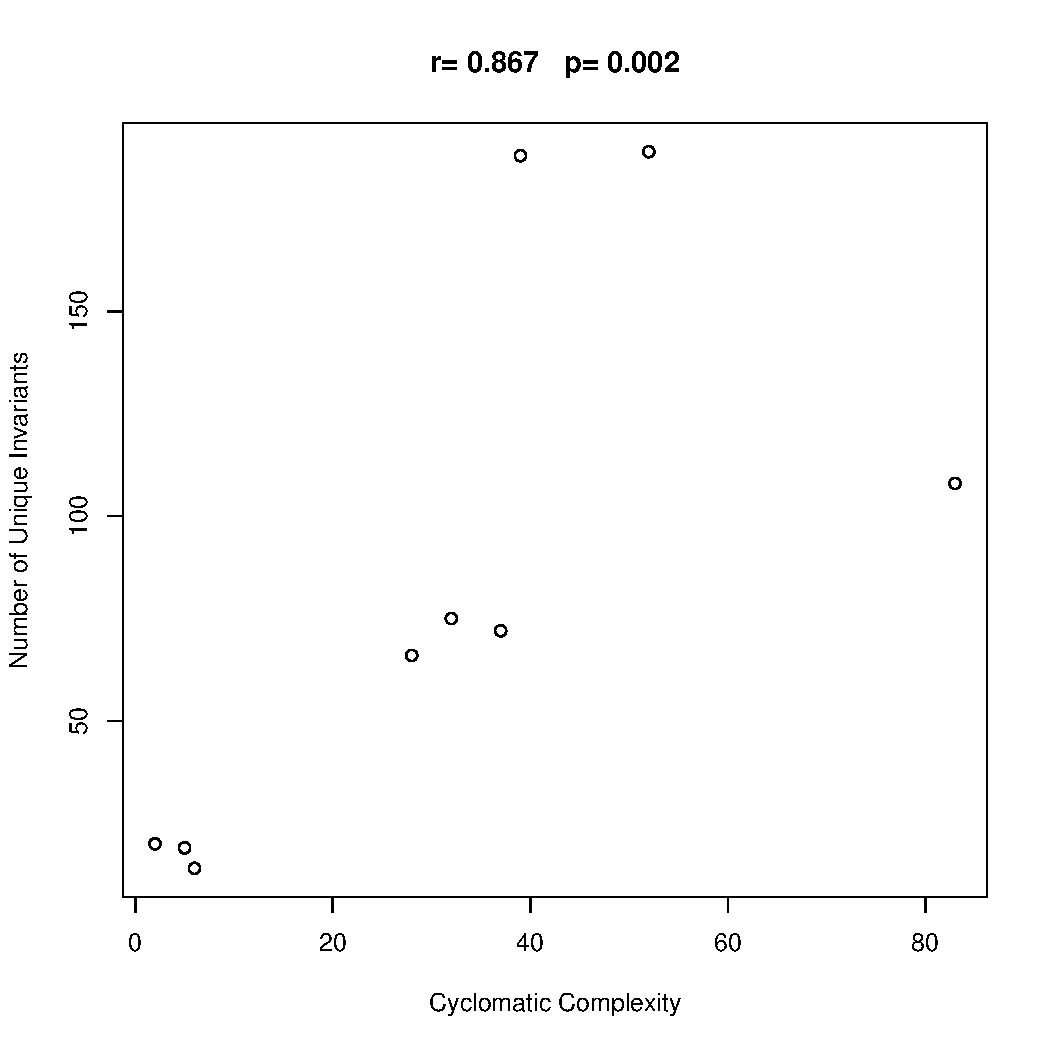
\includegraphics[width=0.7\hsize]{rscripts/inv_cc}
% \mycaption{Scatter plot of the number of unique invariants versus
% cyclomatic complexity. r represents the Spearman correlation coefficient and p is
% the p-value.}
% \label{Fig:inv-cc}
% \vspace{-0.3in}
% \end{figure}
%(1) the precision of comparing two floating point numbers in Daikon;
%The first is concerned with the number of digits in the fractional part of the floating point numbers, which is used by Daikon while comparing two floats. We resolve this by increasing the precision of float comparisons in Daikon configurations.
\head{Unstable Assertions.} As mentioned in \secref{filtering}, we observe a few number of unstable invariant assertions initially, which are removed by our filtering mechanism. By analyzing our trace data, we observe
that such unstable assertions arise mainly because of the 
multiple runtime types of \javascript variables.
This is based on the fact that in \javascript it is possible to change the type of a variable at runtime. However, Daikon treats variables as single type, selects the first observed type, and ignores the subsequent types in the trace data. This results in producing a few number of unstable invariant assertions for \javascript.
We remove such unstable assertions in our filtering step. A drawback of removing these assertions, is that our tool might miss a fault during the regression testing phase.
However, according to our observations, such unstable assertions form only around 5\% of the total generated assertions. Thus, we are still able to achieve high accuracy as presented in the previous section.
    
\head{Limitations.} Our approach is not able to detect syntax errors that are present in the \javascript code. Furthermore, tracing DOM manipulations using APIs other than the standard DOM API or jQuery is currently not supported by \jsart.
Further, a regression fault either directly violates an invariant assertion, or it can violate closely 
related assertions, which have been affected by the fault. However, if the tool is not able to infer any invariants in the  affected scope of the error, it fails to detect the fault. This results in observing a low rate of false negatives as illustrated in \secref{evaluation}. 
     
\head{Revisiting the Assumptions.} As we mentioned in \secref{approach}, we assume that the current version of the web application is bug-free. This is based on the fact that in regression testing a gold standard is always needed as a trusted version for comparing the test results against \cite{Binder:2000} to detect regression faults. However, if the original version of the application does contain an error, the generated assertions might reflect the error as well, and as such they are not able to detect the fault. 
Our second assumption states that the program specifications are unlikely to change frequently in revisions. Here we assume that software programs evolve gradually and regression faults are mostly due to small changes. However, if major upgrades occur in subsequent revisions such that the core specification of the application is affected, the inferred invariants from the original version may not be valid any longer and new invariant assertions need to be generated.

% Competent Programmer Hypothesis (CPH) \cite{acree:mutation1979, demillo:computer1978}. It states that programmers tend to develop programs, which are close to the correct version. Therefore,
% regression faults are mostly due to simple faults occur during small changes in the program. These faults made by competent programmers are merely simple faults such that the applications's behavior is not significanlty affected.


 

\begin{table}[t]
%\vspace{5pt}
        \caption{Manual effort imposed by our approach for deriving stable invariant assertions.}
{\scriptsize
    \begin{center}
       
      %  \subtable[Experimental subjects and the corresponding exploration data]
            {
           \begin{tabular}{c|c|c} \hline
\thead{App ID} & \thead{Total Time (min)} & \thead{Manual Effort (min)} \\  \hline \hline

1  & 13  & 4 \\ \hline %535
           
2  & 11.5 & 3 \\ \hline %502

3 & 15.5  & 5 \\ \hline % 639

4  & 11  & 3 \\ \hline %500

5  & 6.5 & 2.5 \\ \hline %227

6  & 9  & 4.5 \\ \hline %214

7  & 7.5  & 3.5 \\ \hline %244

8  & 6.5  & 2 \\ \hline %278

9  & 18 & 13 \\ \hline %266
\hline\end{tabular}\centering
            }
\label{Table:manualEffort_table}
\end{center}
}  
\vspace{-0.2in} 
\end{table}



\head{Automation Level.} While the testing phase of \jsart is fully automated, the navigation part requires some manual effort. Although the crawling is performed automatically, we do need to manually setup the tool with different crawling configurations per application execution.  Moreover, for each application run, we manually look at the size of the invariant output to decide whether more execution traces (and thus more crawling sessions) are needed.
%Thus, manual effort is concerned with tracing and filtering unstable invaraint assertions, where we need to execute the application 
%per crawling configuration. 
%
We present the manual effort involved with detecting stable invariant assertions in \tabref{manualEffort_table}. 
The table shows the total time, which is the duration time of deriving stable assertions including both automatic and manual parts. 
The reported manual effort contains the amount of time required 
for setting up the tool as well as the manual tasks involved with the navigation part.
The results show the average manual effort is less than 5 minutes.




   
\subsection{Threats to Validity} \label{Sec:threatsToValidity}
An external threat to the validity of our evaluation is the limited number of \javascript applications used to measure the effectiveness of our approach. We mitigated this threat by using web applications from various domains, code size, and functionality. Another threat concerns validating failed assertions through manual inspection that can be error-prone. To mitigate this threat, we carefully examine the code in which the assertion failed to make sure that the injected fault was responsible for the assertion failure. Moreover, manual computation of the \javascript slices to measure precision and recall is a time intensive task done by the authors of the paper, and thus we acknowledge that it could be error-prone, although we made every effort to mitigate this threat by precisely examining the application's code.

The regression faults we inject to evaluate the effectiveness of \tool may not be realistic. We mitigate this threat by injecting mutations that represent common \javascript applications faults, as well as using real-world web applications, and test cases written by other developers.


%\section{Related Work} \label{Sec:related}
%\headbf{Test generation} \label{Sec:test-generation}
%Different constraint-solving approaches have been proposed for test generation. For instance, path\-Crawler \cite{williams:edcc05} combines static and dynamic analysis  
%and performs on-the-fly exploration of the input space of the application. 
%Concolic testing has been employed in DART \cite{godefroid:pldi05} and further extended in CUTE \cite{sen:esec-fse05} and PEX \cite{tillmann:tap08}. 
%However, it is not clear how these approaches scale when applied to dynamic web applications.
%Meta-heuristic search approaches have been used as an alternative to constraint-based techniques. Examples of such approaches are Ribeiro \etal \cite{ ribeiro:ast08},
%Fraser \etal \cite{fraser:qsic11} and
%Harman \etal \cite{harman:aosd09}.
%The success of such methods depends on the availability
%of appropriate fitness functions that can properly guide the solution towards an optimal one \cite{malburg:ase11}. Devising such a fitness function is a significant challenge. 
%To overcome the drawbacks of search-based approaches, Malburg \etal \cite{malburg:ase11} propose to combine constraint-based and search-based testing. 
%The focus of these techniques is mostly on input generation to efficiently cover every possible program flow. 
%In our work, we focus on maximizing the function coverage of the program instead of state space coverage,  as  determining the state space size of dynamic web applications is an undecidable problem.  Further, instead of generating inputs data, we create test oracles capable of detecting faults.

\headbf{Web application testing}
Marchetto and Tonella \cite{marchetto:search} propose a search-based algorithm for generating event-based sequences to test Ajax applications. 
Mesbah et al.  \cite{mesbah:tweb11} apply dynamic analysis to construct a model of the application's state space, from which event-based test cases are automatically generated. They propose \cite{mesbah:tse12} generic and application-specific invariants as a form of automated soft oracles for testing \ajax applications.  Our earlier work, \jsart \cite{mirshokraie:icwe12},  automatically infers program invariants from \javascript execution traces and uses them as regression assertions in the code. 
Sen \etal \cite{sen:fse13} recently proposed a record and replay framework called Jalangi. It incorporates selective record-replay as well as shadow values and shadow execution to enable writing of heavy-weight dynamic analyses.
The framework is able to track generic faults such as \code{null} and \code{undefined} values as well as type inconsistencies in \javascript. 
Jensen \etal \cite{jensen:fse13} propose a technique to test the correctness of communication patterns between client and server in \ajax applications by incorporating server interface descriptions.
They construct server interface descriptions through an inference technique that can learn communication patterns from sample data.
Saxena \etal \cite{song:symb10} combine random test generation with the use of symbolic execution for systematically exploring a \javascript application's event space as well as its value space, for security testing.  Perhaps the most closely related work to ours is \artemis \cite{artzi:icse11}, which supports automated testing of \javascript applications.
\artemis considers the event-driven execution model of a \javascript application for feedback-directed testing.
In this paper, we quantitatively compare our approach with that of \artemis (Section \ref{Sec:evaluation}). 

Our work is different in two main aspects from these works: (1) they all target the generation of event sequences at the DOM level, while we also generate unit tests at the \javascript code level, which enables us to cover more and find more faults,
and (2) they do not address the problem of test oracle generation and only check against soft oracles (e.g., invalid HTML). In contrast, we generate strong oracles that capture
application behaviours, and can detect a much wider range of faults.

\headbf{Oracle generation} \label{Sec:oracleGen}
There has been limited work on oracle generation for testing. 
Fraser \etal \cite{fraser:tse12} propose $\mu$TE\-ST, which employs a mutant-based oracle generation technique.  It automatically generates unit tests for Java object-oriented classes by using a genetic algorithm to target mutations with high impact on the application's behaviour. They further identify~\cite{fraser:issta11} relevant pre-conditions on the test inputs and post-conditions on the outputs to ease human comprehension.
%\shabnam{differential test generation added for issta}
Differential test case generation approaches \cite{taneja:ase08, elbaum:tse09} are similar to mutation-based techniques in that they aim to generate test cases that show the difference between two versions of a program. However, mutation-based techniques such as ours, do not require two different versions of the application.
Rather, the generated differences are in the form of controllable mutations that can be used to generate test cases capable of detecting
regression faults in future versions of the program.
%\karthik{So what's the advantage of having the differences in the form of controllable mutations ?}
Staats \etal \cite{staats:icse11} address the problem of selecting oracle data,  which is formed as a subset of internal state variables as well as outputs for which the expected values are determined.
They apply mutation testing to produce oracles and rank the inferred oracles in terms of their fault finding capability.
This work is different from ours in that they merely focus on supporting the creation of test oracles by the programmer, rather than fully automating the process of test case generation. Further, (1) they do not target \javascript; 
(2) in addition to the code-level mutation analysis, we propose DOM-related mutations to capture error-prone \cite{Ocariza:esem2013} dynamic interactions of \javascript with the DOM.  



\section{Conclusions} \label{Sec:concs}
In this paper, we present an automated technique to generate unit-level assertions for the \javascript code. Given (1) a web application that highly interact with the DOM through the underlying \javascript code, and (2) a DOM-based test suite, we make use of the human-written DOM-based test cases to generate effective assertions that can capture regression faults in the \javascript code. We implemented our approach in an open-source tool called \tool. We empirically evaluated \tool on seven web applications. The results show that our approach (1) is accurate in mapping the assertions to the\javascript code, (2) is effective in detecting injected regression faults (63\% on average), (3) outperforms human-written DOM-based assertions in terms of fault finding capability by 31\% on average, and (4) generates unit assertions that are more effective (26\% on average) than those produced by mutation-based technique.

The results indicate that existing DOM-based test assertions can be leveraged to generate unit-level assertions, however, in our current approach we rely on parts of the code that are covered by the human-written test cases. Our future work will include using learning-based techniques to generate unit-level assertions for parts of the code, that are not examined through existing human-written tests.     

